% Created 2018-04-09 Mon 22:36
% Intended LaTeX compiler: pdflatex
\documentclass[11pt]{article}
\usepackage[utf8]{inputenc}
\usepackage[T1]{fontenc}
\usepackage{graphicx}
\usepackage{grffile}
\usepackage{longtable}
\usepackage{wrapfig}
\usepackage{rotating}
\usepackage[normalem]{ulem}
\usepackage{amsmath}
\usepackage{textcomp}
\usepackage{amssymb}
\usepackage{capt-of}
\usepackage{hyperref}
\usepackage{amssymb}
\DeclareMathOperator*{\argmax}{arg\,max}
\usepackage{istgame}
\DeclareMathOperator*{\argmin}{arg\,min}
\usepackage{color}
\date{\today}
\title{}
\hypersetup{
 pdfauthor={},
 pdftitle={},
 pdfkeywords={},
 pdfsubject={},
 pdfcreator={Emacs 26.0.91 (Org mode 9.1.6)}, 
 pdflang={English}}
\begin{document}

\tableofcontents


\section{Entscheidungstheorie}
\label{sec:orge5d4a7d}
\subsection{Naive Entscheidungsregeln / Entscheidung unter Ungewissheit}
\label{sec:org31eef64}
Als Entscheidung unter Ungewissheit bezeichnet man Entscheidungssituationen, bei denen zwar die Alternativen(Strategien), die möglichen Umweltzustände und die Ergebnisse bei Wahl einer bestimmten Alternative und Eintritt eines bestimmten Umweltzustandes bekannt sind, die \emph{Eintrittswahrscheinlichkeiten der Umweltzustände} jedoch \emph{ubekannt} sind.\\
Beispiel Aufgabe: \emph{Person besitzt 100\texteuro{} und muss sich zwischen zwei Strategien s \(\epsilon\) S (= s\(_{\text{1}}\) , s\(_{\text{2}}\)) entscheiden. Es gibt zwei Umweltzustände z \(\epsilon\) Z (= z\(_{\text{1}}\), z\(_{\text{2}}\)). Welche Strategie wählt die Person je nach angewendetem Entscheidungskriterium, wenn sie sich für \textbf{eine} Strategie entscheidet?}\\
\newline
1.) Erstelle Auszahlungsmatrix\\
m = Kapital der Person = 100\texteuro{}\\
\(\pi\) = Auszahlungsfunktion die von Strategie s und Umweltzustand z abhängt und eine dementsprechende Auszahlung angibt: Wenn s\(_{\text{1}}\) für Umweltzustand z\(_{\text{1}}\) eine Steigerung des Vermögens um 40\% garantiert und für Umweltzustand s\(_{\text{2}}\) -20\%, dann betragen die jeweiligen Auszahlungen die in die Auszahlungsmatrix gehören:

\begin{equation*}
\begin{aligned}
\pi(s_1,z_1)=m*(1+0.4)=100*1.4=140\\
\pi(s_1,z_2)=m*(1-0.2)=100*0.8=80
\end{aligned}
\end{equation*}
Für s\(_{\text{2}}\) , bei z\(_{\text{1}}\) -10\% und für z\(_{\text{2}}\) 20\%, betragen die Auszahlungen demnach:
\begin{equation*}
\begin{aligned}
\pi(s_2,z_1)=100*0.9=90\\
\pi(s_2,z_2)=100*(1+0.2)=120
\end{aligned}
\end{equation*}
Auszahlungsmatrix:
\begin{center}
\begin{tabular}{c|c|c}
s\textbackslash{z} & z\(_{\text{1}}\) & z\(_{\text{2}}\)\\
\hline
s\(_{\text{1}}\) & 100*1.4=140 & 100*0.8=80\\
s\(_{\text{2}}\) & 100*0.9=90 & 100*1.2=120\\
\end{tabular}
\end{center}
Bei einer möglichen Mischanlage oder Mischwahl wird die Auszahlungsmatrix um eine Zeile(Mischstrategie erweitert):
\begin{center}
\begin{tabular}{c|c|c}
s\textbackslash{z} & z\(_{\text{1}}\) & z\(_{\text{2}}\)\\
\hline
s\(_{\text{1}}\) & 100*1.4=140 & 100*0.8=80\\
MS & 140*\(\alpha\) + (1-\(\alpha\))*90 & 80*\(\alpha\) + (1-\(\alpha\))*120\\
s\(_{\text{2}}\) & 100*0.9=90 & 100*1.2=120\\
\end{tabular}
\end{center}
\(\alpha\) beschreibt den Anteil der in s\(_{\text{1}}\) investiert wird, demnach fließt 1-\(\alpha\) in s\(_{\text{2}}\) fuer jeden Umweltzustand
\newline
2.) Strategie Wahl\\
Entscheidungsregeln: Maximin, Maximax, Hurwics, Regel des minimalen Bedauerns, Laplace\\
\subsubsection{Maximin (Pessimist)}
\label{sec:orge32e6fc}
Immer vom schlechtesten Fall ausgehen(risikoavers). Wähle daher die Strategie s \(\epsilon\) S mit dem \textbf{größtem} Zeilen\textbf{minimum}:\\
\(\displaystyle Zeilenminimum = \min_{z \epsilon Z} \pi(s,z)\)
\newline
\(\displaystyle Zeilenminimum_{s_1} = \min_{z \epsilon Z} \pi(s_1,z)\)
\newline
\(\displaystyle Zeilenminimum_{s_2} = \min_{z \epsilon Z} \pi(s_2,z)\)

Betrachte also fuer jede Strategie alle Auszahlungen fuer die jeweiligen Umweltzustände z \(\epsilon\) Z und suche pro Strategie die kleinste Auszahlung:\\
Fuer s\(_{\text{1}}\) beispielsweise: \(\pi\)(s\(_{\text{1}}\), z\(_{\text{1}}\)) = 140 und \(\pi\)(s\(_{\text{1}}\), z\(_{\text{2}}\)) = 80 \(\rightarrow\) 
\(\displaystyle \min_{z \epsilon Z} \pi(s_1,z) = 80\)
\newline
Und fuer die zweite Strategie: \(\displaystyle \min_{z \epsilon Z} \pi(s_2,z) = 90\)
\newline
Finde nun das Maximum der Zeilenminima der Strategien um die optimale Strategie nach der Maximin-Regel herauszufinden:
\(\displaystyle \argmax_{s \epsilon S}\min_{z \epsilon Z} \pi(s,z) = \argmax_{s \epsilon S}(80,90) = \arg(90) = s_2\)
\newline
\(\rightarrow\) Nach der Maximin-Regel wählt die Person s2, da s2 im "schlimmsten" Falls das "beste" Ergebnis liefert.\\

 \textbf{Mischanlage}\\
Setze MS\(_{\text{z}_{\text{1}}}\) und MS\(_{\text{z}_{\text{2}}}\) gleich und löse nach \(\alpha\) auf:\\
\begin{equation*}
\begin{aligned}
&140*\alpha + (1-\alpha)*90 = 80*\alpha + (1-\alpha)*120\\
&140\alpha - 90\alpha + 90 = 80\alpha - 120\alpha +120\\
&50\alpha + 90 = -40 \alpha + 120\\
&90\alpha = 30\\
&\alpha = \frac{3}{9} = \frac{1}{3}
\end{aligned}
\end{equation*}
Bei Maximin wird \(\alpha = \frac{1}{3}\) gewählt, da dieses \(\alpha\) unabhängig vom eintretenden Umweltzustand für beide Strategien die selbe Auszahlung(einsetzen) ergibt.
\newline
\subsubsection{Maximax (Optimist)}
\label{sec:org583ca08}
Immer vom besten Fall ausgehen(risikofreudig). Wähle daher die Strategie s mit dem \textbf{größtem} Zeilen\textbf{maximum}:\\
\(\displaystyle Zeilenmaximum = \max_{z \epsilon Z} \pi(s,z)\)
\newline
Die optimale Strategie s* ergibt sich nach der Maximax-Regel wie folgt:\\
\(\displaystyle s^* = \argmax_{s \epsilon S} \max_{z \epsilon Z} \pi(s,z)\)
\newline
\textbf{Mischanlage}\\
Da risikofreudig einmal \(\alpha=0\) und \(\alpha=1\) in beide Mischstrategien einsetzen und maximale Auszahlung bei \(\alpha\) = 0 und \(\alpha\) = 1 ermitteln und dann wiederum das Maximum der beiden Maxima ermitteln.\\
\(\alpha\) = 0:\\
\begin{equation*}
\begin{aligned}
&MS_{z_1}=140*0 + (1-0)*90 = 90\\
&MS_{z_2}=80*0 + (1-0)*120 = 120
\end{aligned}
\end{equation*}
\newline
\(\alpha\) = 1:\\
\begin{equation*}
\begin{aligned}
&MS_{z_1}=140*1 + (1-1)*90 = 140\\
&MS_{z_2}=80*1 + (1-1)*120 = 80
\end{aligned}
\end{equation*}
\newline
\(\rightarrow\) \(\max(120,140)=140\) \(\rightarrow\) wähle \(\alpha\) = 1, da dort das größte Maximum möglich ist.
\newline\\
\subsubsection{Hurwics}
\label{sec:org40a15ce}
Ist eine Mischform aus Optimismus und Pessimismus und wird daher mithilfe des "Optimismuskoeffizienten" \(\gamma\) berechnet:\\
\(\displaystyle s^* = \argmax_{s \epsilon S}(\gamma * \max_{z \epsilon Z} \pi(s,z) + (1 - \gamma) * \min_{z \epsilon Z} \pi(s,z))\)
\newline
Vorgehen: 
\(\displaystyle \gamma * \max_{z \epsilon Z} \pi(s,z) + (1 - \gamma) * \min_{z \epsilon Z} \pi(s,z)\) für jede Strategie ausfüllen (also den Optimismuskoeffizienten \(\gamma\) mal den "besten" Fall plus 1 minus \(\gamma\) mal den schlechten Fall für jede Strategie):\\
\begin{equation*}
\begin{aligned}
s_1: \gamma * 140 + 1 - \gamma * 80\\
s_2: \gamma * 120 + 1 - \gamma * 90
\end{aligned}
\end{equation*}
Danach beide Formeln gleichsetzen und nach \(\gamma\) auflösen, um das \(\gamma\) zu finden bei dem die erwarteten Auszahlungen gleich und die Person indifferent zwischen beiden Strategien ist
\begin{equation*}
\begin{aligned}
&\gamma * 140 + (1 - \gamma) * 80 = \gamma * 120 + (1 - \gamma) * 90\\
&140\gamma - 80\gamma + 80 = 120\gamma - 90\gamma + 90\\
&60\gamma + 80 = 30\gamma + 90\\
&30\gamma = 10\\
&\gamma = \frac{10}{30} = \frac{1}{3}
\end{aligned}
\end{equation*}
Bei \(\gamma=\frac{1}{3}\) ist die Person indifferent zwischen s\(_{\text{1}}\) und s\(_{\text{2}}\), da bei beiden Strategien eine Auszahlung von 100 zu erwarten ist. Für \(\gamma<\frac{1}{3}\) liefert s\(_{\text{2}}\) höhere Auszahlungen (rausfinden durch einsetzen) und fuer \(\gamma>\frac{1}{3}\) ist s\(_{\text{1}}\) die bessere Wahl.\\
\[ s^* =\begin{cases} 
      s_2 & \gamma < \frac{1}{3} \\
      indifferent & \gamma=\frac{1}{3} \\
      s_1 & \gamma > \frac{1}{3}
   \end{cases}
\]
\newline
\textbf{Mischanlage}\\
Mischung aus Pessimist(bei dem \(\alpha = \frac{1}{3}\)) war und Optimist bei dem \(\alpha\) = 1 war. Mischstrategie für beide Umweltzustände mit beiden \(\alpha\)'s einsetzen. Dann für beide Auszahlungen des jeweiligen Alpha, die höhere Auszahlung mal \(\gamma\) plus die niedrigere Auszahlung mal 1 minus \(\gamma\) und so weit wie möglich ausmultiplizieren.\\
\(\alpha = \frac{1}{3}\): \\
\begin{equation*}
\begin{aligned}
&MS_{z_1}=140*\frac{1}{3} + \frac{2}{3}*90=\frac{320}{3}\\
&MS_{z_2}=80*\frac{1}{3} + \frac{2}{3}*120=\frac{320}{3}\\
\rightarrow \frac{320}{3}*\gamma + (1-\gamma)*\frac{320}{3} = \frac{320}{3}
\end{aligned}
\end{equation*}

\(\alpha = 1\): \\
\begin{equation*}
\begin{aligned}
&MS_{z_1}140*1 + (1-1)*90=140\\
&MS_{z_2}80*1 + (1-1)*120=80\\
\rightarrow 140*\gamma + (1-\gamma)*80 = 60\gamma+80
\end{aligned}
\end{equation*}

Die beiden daraus resultierenden Gleichungen nun gleichsetzen und nach Gamma auflösen:\\
\begin{equation*}
\begin{aligned}
60\gamma+80 = \frac{320}{3}\\
60\gamma = \frac{80}{3}\\
\gamma = \frac{4}{9}
\end{aligned}
\end{equation*}

Bei diesem \(\gamma = \frac{4}{9}\) ist die Person indifferent zwischen Pessimismus (\(\alpha = \frac{1}{3}\)) und Optimismus (\(\alpha\) =1)\\
\[ \alpha =\begin{cases} 
      \frac{1}{3} & \gamma < \frac{4}{9} \\
      {\frac{1}{3},1} & \gamma=\frac{4}{9} \\
      1 & \gamma > \frac{4}{9}
   \end{cases}
\]
\newline\\
\subsubsection{Regel des minimalen Bedauerns}
\label{sec:orgac2b4c4}
Überführe die Auszahlungsmatrix in eine "Bedauernsmatrix": "Wieviel geht mir durch die Lappen wenn der jeweils schlechtere Zustand eintritt?" \(\rightarrow\) Differenz zum Spaltenmaximum bilden und eintragen und für Spaltenmaximum = 0:\\
\begin{center}
\begin{tabular}{c|c|c}
s\textbackslash{z} & z\(_{\text{1}}\) & z\(_{\text{2}}\)\\
\hline
s\(_{\text{1}}\) & 140 & 80\\
s\(_{\text{2}}\) & 90 & 120\\
\end{tabular}
\end{center}
wird zur Bedauernsmatrix:
\begin{center}
\begin{tabular}{c|c|c}
s\textbackslash{z} & z\(_{\text{1}}\) & z\(_{\text{2}}\)\\
\hline
s\(_{\text{1}}\) & 0 & 40\\
s\(_{\text{2}}\) & 50 & 0\\
\end{tabular}
\end{center}
Wähle dann die Strategie mit dem geringsten Bedauern, also die Strategie mit dem kleinsten Zeilenmaximum\\
\(\displaystyle s^* = \argmin_{s \epsilon S}\max_{z \epsilon Z} = \argmin_{s \epsilon S}(40, 50) = \arg(40) = s_1\)
\newline\\
\textbf{Mischanlage}\\
Ziehe die Mischstrategie vom Spaltenmaximum ab (für alle Umweltzustände) um das Bedauern festzustellen.

\begin{equation*}
\begin{aligned}
z_1: 140 - (140*\alpha + (1-\alpha)*90) = 50\alpha +90 \\
z_2: 120 - (80*\alpha + (1-\alpha)*120) = -40\alpha+120
\end{aligned}
\end{equation*}

Setze die daraus resultierenden Gleichungen gleich und löse nach \(\alpha\) auf um das \(\alpha\) zu erhalten, bei dem das Bedauern unabhängig vom eintretenden Umweltzustand gleich ist.

\begin{equation*}
\begin{aligned}
 50\alpha +90 = -40\alpha+120\\
90\alpha = 30\\
\alpha = \frac{1}{3}
\end{aligned}
\end{equation*}

\(\rightarrow\) Er wählt \(\alpha = \frac{1}{3}\) um das Bedauern unabhängig vom Umweltzustand zu minimieren

\subsubsection{Laplace}
\label{sec:org3b72c9a}
Annahme, dass alle Umweltzustände mit der gleichen Wahrscheinlichkeit auftreten (bei zwei Umweltzuständen jeweils 50\%). Daher Bildung der durchschnittlich zu erwartenden Auszahlung:
\begin{equation*}
\begin{aligned}
s_1: (140 + 80) * 0.5 = 110 \\
s_2: (90+120)*0.5=105
\end{aligned}
\end{equation*}
\(\rightarrow\) Wähle s\(_{\text{1}}\) weil höherer Erwartungswert.
\newline

\textbf{Mischanlage}\\
Bilde die durchschnittlich zu erwartende Auszahlung der Mischstrategie: \(MS_{z_1}*0.5+MS_{z_2}*0.5\)

\begin{equation*}
\begin{aligned}
&0.5*(140*\alpha + (1-\alpha)*90) + 0.5*(80*\alpha + (1-\alpha)*120) \\ 
&= 0.5*(50\alpha + 90) + 0.5*(-40\alpha + 120)\\ 
&= 25\alpha + 45 - 20\alpha + 60\\
&= 5\alpha + 105
\end{aligned}
\end{equation*}

\(\rightarrow\) \(5\alpha + 105\) wird maximiert wenn \(\alpha\) = 1 ist, daher wähle \(\alpha\) = 1 was die gesamte Fokussierung auf s\(_{\text{1}}\) bedeutet.\\

\subsection{Entscheidungen unter Risiko}
\label{sec:org02dda8f}
Entscheidungen unter Risiko entscheiden sich von Entscheidungssituationen unter Ungewissheit insofern, dass man davon ausgehen kann, dass die Wahrscheinlichkeiten für das Eintreten bestimmter Umweltzustände als bekannt vorausgesetzt werden. \\
\subsubsection{Bayes Regel}
\label{sec:orgac9d73c}
Zu den Entscheidungsregeln in solchen Szenarien zählt die \textbf{Bayes-Regel}. Diese sagt aus, dass der Entscheider sich nur nach den Erwartungswerten orientiert. Man multipliziert hierzu die Wahrscheinlichkeit des jeweiligen Zustandes mit der dazugehörigen Auszahlung und addiert dies, um den Erwartungswert für eine Strategie zu erhalten. Dabei ist zu beachten das die Auszahlung zuvor in die Nutzenfunktion des Entscheiders eingesetzt werden muss.\\

Beispiel: \emph{Die Wahrscheinlichkeit von z\(_{\text{1}}\) beträgt 75\%, von w\(_{\text{2}}\) 25\%.} 
\begin{center}
\begin{tabular}{c|c|c}
W & w\(_{\text{1}}\)=75\% & w\(_{\text{2}}\)=25\%\\
\hline
S\textbackslash{Z} & z\(_{\text{1}}\) & z\(_{\text{2}}\)\\
\hline
s\(_{\text{1}}\) & 100 & 81\\
s\(_{\text{2}}\) & 78 & 151\\
\end{tabular}
\end{center}
\textbf{Risikoneutraler Entscheider}:\\
(lineare) Nutzenfunktion \(u(\pi)=\pi\), E\(_{\text{i}}\) Erwartungswert von Strategie i

\begin{equation*}
\begin{aligned}
E(u(\pi))_{s_1} = 0.75*u(100) + 0.25*u(81) = 0.75 * 100 + 0.25*81=95.25\\
E(u(\pi))_{s_2}= 0.75*u(74) + 0.25*u(141) = 0.75*78 + 0.25*151 = 96.25
\end{aligned}
\end{equation*}
\(\rightarrow\) Wenn der Entscheider risikoneutral ist würde er sich für Strategie s\(_{\text{2}}\) entscheiden, da diese den höheren Erwartungswert hat.\\
\textbf{Risikoscheuer Entscheider}:\\
Nutzenfunktion \(u(\pi)=\sqrt{\pi}\), E\(_{\text{i}}\) Erwartungswert von Strategie i

\begin{equation*}
\begin{aligned}
E(u(\pi))_{s_1} = 0.75*u(100) + 0.25*u(81) = 0.75 * \sqrt{100} + 0.25*\sqrt{81}=9.75\\
E(u(\pi))_{s_2}= 0.75*u(74) + 0.25*u(141) = 0.75*\sqrt{78} + 0.25*\sqrt{151} = 9.70
\end{aligned}
\end{equation*}
\(\rightarrow\) Wenn der Entscheider risikoavers ist würde er sich für Strategie s\(_{\text{1}}\) entscheiden, da diese den höheren Erwartungswert hat. Grund: s\(_{\text{2}}\) hat zwar an sich den höheren Erwartungswert (siehe risikoneutral) ist aber riskanter.

\subsubsection{Sicherheitsäquivalent \& Risikoprämie}
\label{sec:org14923b7}
Das Sicherheitsäquivalent einer unsicheren Zahlung ist der Betrag einer äquivalenten sicheren Zahlung:
\(u(SÄ) = E(u(\pi))\) . Der Wert des SÄ hängt dementsprechend direkt von der individuellen Nutzenfunktion u(\(\pi\)) des Entscheiders ab.

Beispiel: Lineare Nutzenfkt \(u(\pi)=\pi\) \\
\begin{equation*}
\begin{aligned}
E(u(\pi))_{s_1} = 95.25 == u(\textnormal{SÄ}) \rightarrow \textnormal{SÄ} = 95.25\\
E(u(\pi))_{s_2} = 96.25 == u(\textnormal{SÄ}) \rightarrow \textnormal{SÄ} = 96.25
\end{aligned}
\end{equation*}
weil \(u(\pi) == \pi\) ist \(95.25 == u(95.25)\) \\

Beispiel: Wurzel-Nutzenfkt \(u(\pi)=\sqrt{\pi}\) \\
\begin{equation*}
\begin{aligned}
E(u(\pi))_{s_1} = 9.75 == u(\textnormal{SÄ}) \rightarrow u(\textnormal{SÄ}) = 9.75 \rightarrow \sqrt{\textnormal{SÄ}}=9.75 \rightarrow \textnormal{SÄ}= 95.06\\
E(u(\pi))_{s_2} = 9.70 == u(\textnormal{SÄ}) \rightarrow u(\textnormal{SÄ}) = 9.70 \rightarrow \sqrt{\textnormal{SÄ}}=9.70 \rightarrow \textnormal{SÄ}= 94.09
\end{aligned}
\end{equation*}\\
\newline
Die Risikoprämie ist die Differenz zwischen dem Erwartungswert und dem Sicherheitsäquivalent. Sie misst wie viel dem Entscheider die Eliminierung des Risikos wert ist.\\
Beispiel: Lineare Nutzenfkt $u(\pi)=\pi$ \\
Erwartungswert entspricht dem Sicherheitsäquivalent daher ist Risikoprämie = 0.\\
Beispiel: Wurzel-Nutzenfkt $u(\pi)=\sqrt{\pi}$ \\
\begin{equation*}
\begin{aligned}
RP_{s_1}= E(\pi)_{s_1} - \textnormal{SÄ} = 95.25 - 95.06 = 0.19 \\
RP_{s_2}= E(\pi)_{s_2} - \textnormal{SÄ} = 96.25 - 94.09 = 2.16 \\
\end{aligned}
\end{equation*}

\subsubsection{Bernoulli Prinzip}
\label{sec:org3ec4c0c}
Sankt-Petersburg-Paradoxon stellt Bayes Regel in Frage. Es zeigt, dass die Berücksichtigung von Erwartungswerten nicht in allen Fällen dem Entscheidungsverhalten von Menschen in der Realität entspricht (Beispiel Münzwurf 1\texteuro{} wenn Kopf beim ersten Wurf, 2\texteuro{}  wenn Kopf beim zweiten Wurf, 4\texteuro{}  wenn Kopf beim dritten Wurf, 2\(^{\text{n-1}}\)\texteuro{} wenn Kopf beim n-ten Wurf \(\rightarrow\) Erwartungswert = \(\infty\) \(\rightarrow\) Individum würde sein gesamtes Vermögen einsetzen, um an der Lotterie teilzunehmen?!).\\
Das Bernoulli Prinzip löst jenes Paradoxon und gilt als rationales Entscheidungskriterium.\\
Annahme des BP: Der Spieler hat eine Wurzel-Nutzenfunktion, somit wäre der erwartete Nutzen:\\
\begin{equation*}
\begin{aligned}
E(u(\pi))=\frac{1}{2}*\sqrt{1} +\frac{1}{4}*\sqrt{2} +\frac{1}{8}*\sqrt{4} + ... \approx 1.71\\
\end{aligned}
\end{equation*}
\(\rightarrow\)  entspricht einer sicheren Zahlung (SÄ) von 2.91, da:\\
\(1.71 = \sqrt{\textnormal{SÄ}} \rightarrow 1.71 = \sqrt{2.91} \rightarrow \textnormal{SÄ} = 2.91\) \\
Somit wäre der Spieler bereit einen endlichen Betrag für die Lotterie zu zahlen, was realistischer ist.

\subsubsection{Maße für Risikoaversion}
\label{sec:org30da9c4}
Individuen mit \textbf{konkaver} (\(\frown\), zweite Ableitung < 0) Nutzenfunktion sind risikoavers. Es gilt, dass der Erwartungswert des Nutzens kleiner ist als der Nutzen des Erwartungswerts: \(E(u(\pi)) < u(E(\pi)\) .\\
Individuen mit \textbf{konvexer} (\(\smile\), zweite Ableitung > 0) Nutzenfunktion sind risikofreudig. Es gilt, dass der Erwartungswert des Nutzens größer ist als der Nutzen des Erwartungswerts: \(E(u(\pi)) > u(E(\pi)\) .\\
Individuen mit \textbf{linearer} (---) Nutzenfunktion sind risikofreudig. Es gilt, dass der Erwartungswert des Nutzens und der Nutzen des Erwartungswerts übereinstimmen.\\
Beispiel:
\(E(\pi)_{s_1} = 100 *0.4 + 60 * 0.6 = 76\) \\
\textbf{bei risikoaverser Nutzenfkt \(u(\pi)=\sqrt{\pi}\) :}\\
\begin{equation*}
\begin{aligned}
&E(u(\pi))_{s_1} = \sqrt{100} * 0.4 + \sqrt{60} 0.6 = 8.65 \\
&u(E(\pi))_{s_1}= \sqrt{E(\pi)} = \sqrt{76} =8.72 \\
&\rightarrow E(u(\pi)) < u(E(\pi) \rightarrow 8.65 < 8.72 \checkmark\\
\end{aligned}
\end{equation*}
Bedeutet dass der Entscheider eine sichere Zahlung in Höhe von E(\(\pi\)) besser als eine Lotterie mit dem gleichen Erwartungswert findet.\\
\newline
\textbf{bei risikofreudiger Nutzenfkt \(u(\pi)=\pi^2\) :} \\
\begin{equation*}
\begin{aligned}
&E(u(\pi))_{s_1} = 100^2 * 0.4 + 60^2 * 0.6 = 6160 \\
&u(E(\pi))_{s_1}= {E(\pi)}^2 = {76}^2 =5776 \\
&\rightarrow E(u(\pi)) > u(E(\pi) \rightarrow 6160 > 5776 \checkmark\\
\end{aligned}
\end{equation*}
\newline
Wie kann man die Stärke der Risikoaversion messen?
\paragraph{Absolute Risikoaversion}
\(ARA(\pi)= -\frac{u''(\pi)}{u'(\pi)}\) ist unabhängig vom Anfangsvermögen des Entscheiders (Entscheidungen sind in diesem Sinne \textbf{absolut}). Wenn ARA konstant, dann konstante \textbf{absolute} Risikoaversion.\\
\paragraph{Relative Risikoaversion}
\(RRA(\pi)= -\pi * \frac{u''(\pi)}{u'(\pi)}\) wird durch Anfangsvermögen des Entscheiders \textbf{relativiert}. Wenn RRA konstant, dann hat der Entscheider eine konstante \textbf{relative} Risikoaversion\\
\subsection{Dynamische Entscheidungen}
\label{sec:org3aaead1}
Beispiel:\\
\begin{istgame}[scale=1.5,font=\footnotesize]
\xtdistance{15mm}{43mm}
\istroot(0){Anfangsknoten}
  \istb{Investition}[al]
  \istb{keine Investition}[ar]
  \endist
\xtdistance{15mm}{20mm}
\istroot(1)(0-1)<180>{}
  \istb{Marketing}[l]
  \istb{kein Marketing}[r]
  \endist
\istroot(2)(0-2)<0>{}
  \istb{Marketing}[l]
  \istb{kein Marketing}[r]
  \endist
\xtdistance{15mm}{10mm}
\istroot(a)(1-1)<180>{10}
  \endist
\istroot(b)(1-2)<0>{5}
  \endist
\istroot(c)(2-1)<180>{6}
  \endist
\istroot(d)(2-2)<0>{7}
\endist
\end{istgame}    
\newline
Lösung über Rückwärtsinduktion: Betrachte Teilbäume des eigentlichen Entscheidungsbaum und treffe Entscheidung, lasse dann die Kanten des betrachteten Teilbaums fallen und schreibe den Nutzen der gewählten Entscheidung an seinen Knoten:\\
\begin{istgame}[scale=1.5,font=\footnotesize]
\xtdistance{5mm}{20mm}
\istroot(0){Anfangsknoten}
  \istb{Investition}[al]
  \istb{keine Investition}[ar]
  \endist
\xtdistance{5mm}{10mm}
\istroot(1)(0-1)<180>{10}
  \endist
\istroot(2)(0-2)<0>{7}
  \endist
\end{istgame}    

\paragraph{Perfekte Information, aber Züge der Natur}
Ist konzeptionell genau identisch zum obigen, grundlegenden Fall(perf Inf, keine Züge der Natur). Der einzige Unterschied ist, dass die Natur zwischendurch zieht und somit Unsicherheit/Risiko ins Spiel bringt. Deshalb wendet man die Konzepte des Entscheidens unter Unsicherheit(Ungewissheit?!)/Risiko am entsprechenden Knoten an.\\
Beispiel: \emph{Regenschirmproduktion gibt bei gutem Wetter(25\%) 9 und bei schlechtem Wetter(75\%) 10. Sonnenschirmproduktion gibt respektive 11 und 8.}\\
\begin{istgame}[scale=1.5,font=\footnotesize]
\xtdistance{5mm}{20mm}
\istroot(0){}
  \istb{R}[al]
  \istb{S}[ar]
  \endist
\xtdistance{7mm}{10mm}
\istroot(1)(0-1)<180>{}
  \istb{g:\frac{1}{4}}[l]
  \istb{s:\frac{3}{4}}[r]
  \endist
\istroot(2)(0-2)<0>{}
  \istb{g:\frac{1}{4}}[l]
  \istb{s:\frac{3}{4}}[r]
  \endist
\xtdistance{15mm}{10mm}
\istroot(a)(1-1)<180>{9}
  \endist
\istroot(b)(1-2)<0>{10}
  \endist
\istroot(c)(2-1)<180>{11}
  \endist
\istroot(d)(2-2)<0>{8}
\endist
\end{istgame}

Der nächste Schritt ist dann, die Kanten der Teilbäume fallen zu lassen und an ihren Knoten den jeweiligen Erwartungs\textbf{nutzen} zu schreiben um so das Spiel nach und nach durch Rückwärtsinduktion zu lösen.\\
Bei \textbf{imperfekter} Information wüsste der Entscheider beispielsweise nicht in welchem Knoten er gerade ist, da er beispielsweise nicht über den Zug der Natur informiert ist.

\section{Spieltheorie}
\label{sec:org7ba76ac}
In der Spieltheorie gibt es im Unterschied zur Entscheidungstheorie eine \textbf{Bimatrix} statt der Auszahlungsmatrix. In dieser sind die Einträge bereits \emph{Nutzengrößen}. Die Unsicherheit existiert nun nicht mehr im Hinblick auf Umweltzustände, sondern im Hinblick auf die Strategie eines weiteren Spielers. Da man nun die Auszahlungen für beide Spieler angeben muss, benötigt man zwei Matrizen \emph{oder} eine mit doppelten Einträgen, also eine "Bimatrix".
\begin{center}
\begin{tabular}{c|c|c|c}
S & s\(^{\text{1}}_{\text{2}}\) & s\(^{\text{2}}_{\text{2}}\) & s\(^{\text{3}}_{\text{2}}\)\\
\hline
s\(^{\text{1}}_{\text{1}}\) & (u\(_{\text{1}}\)(s\(^{\text{1}}_{\text{1,s}}\)\(^{\text{1}}_{\text{2}}\)), u\(_{\text{2}}\)(s\(^{\text{1}}_{\text{1}}\), s\(^{\text{1}}_{\text{2}}\))) & (u\(_{\text{1}}\)(s\(^{\text{1}}_{\text{1,s}}\)\(^{\text{2}}_{\text{2}}\)), u\(_{\text{2}}\)(s\(^{\text{1}}_{\text{1}}\), s\(^{\text{2}}_{\text{2}}\))) & (u\(_{\text{1}}\)(s\(^{\text{1}}_{\text{1,s}}\)\(^{\text{3}}_{\text{2}}\)), u\(_{\text{2}}\)(s\(^{\text{1}}_{\text{1}}\), s\(^{\text{3}}_{\text{2}}\)))\\
s\(^{\text{2}}_{\text{1}}\) & (u\(_{\text{1}}\)(s\(^{\text{2}}_{\text{1,s}}\)\(^{\text{1}}_{\text{2}}\)), u\(_{\text{2}}\)(s\(^{\text{2}}_{\text{1}}\), s\(^{\text{1}}_{\text{2}}\))) & (u\(_{\text{1}}\)(s\(^{\text{2}}_{\text{1,s}}\)\(^{\text{2}}_{\text{2}}\)), u\(_{\text{2}}\)(s\(^{\text{2}}_{\text{1}}\), s\(^{\text{2}}_{\text{2}}\))) & (u\(_{\text{1}}\)(s\(^{\text{2}}_{\text{1,s}}\)\(^{\text{3}}_{\text{2}}\)), u\(_{\text{2}}\)(s\(^{\text{2}}_{\text{1}}\), s\(^{\text{3}}_{\text{2}}\)))\\
s\(^{\text{3}}_{\text{1}}\) & (u\(_{\text{1}}\)(s\(^{\text{3}}_{\text{1,s}}\)\(^{\text{1}}_{\text{2}}\)), u\(_{\text{2}}\)(s\(^{\text{3}}_{\text{1}}\), s\(^{\text{1}}_{\text{2}}\))) & (u\(_{\text{1}}\)(s\(^{\text{3}}_{\text{1,s}}\)\(^{\text{2}}_{\text{2}}\)), u\(_{\text{2}}\)(s\(^{\text{3}}_{\text{1}}\), s\(^{\text{2}}_{\text{2}}\))) & (u\(_{\text{1}}\)(s\(^{\text{3}}_{\text{1,s}}\)\(^{\text{3}}_{\text{2}}\)), u\(_{\text{2}}\)(s\(^{\text{3}}_{\text{1}}\), s\(^{\text{3}}_{\text{2}}\)))\\
\end{tabular}
\end{center}
Die Nummer der Strategie ist nun im Gegensatz zu Kapitel 1 hochgestellt, unten steht die Nummer des Spielers.
\subsection{Beispiele}
\label{sec:org3ed4276}
\subsubsection{Hirschjagd}
\label{sec:orgf27e2e2}
\begin{center}
\begin{tabular}{c|c|c}
\textcolor{magenta}{Jäger 1}/\textcolor{blue}{Jäger 2} & \textcolor{blue}{Hirsch} & \textcolor{blue}{Hase}\\
\hline
\textcolor{magenta}{Hirsch} & (\textcolor{magenta}{5},\textcolor{blue}{5}) & (\textcolor{magenta}{0},\textcolor{blue}{4})\\
\textcolor{magenta}{Hase} & (\textcolor{magenta}{4},\textcolor{blue}{0}) & (\textcolor{magenta}{4},\textcolor{blue}{4})\\
\end{tabular}
\end{center}
\subsubsection{Kopf oder Zahl}
\label{sec:orgc055dea}
Jeder Spieler legt unbeobachtbar für den anderen Spieler eine Münze, stimmen die Bilder überein erhält Spieler 1 die Münzen, unterscheiden sie sich so erhält Spieler 2 die Münzen.
\begin{center}
\begin{tabular}{c|c|c}
\textcolor{magenta}{Spieler 1}/\textcolor{blue}{Spieler 2} & \textcolor{blue}{Kopf} & \textcolor{blue}{Zahl}\\
\hline
\textcolor{magenta}{Kopf} & (\textcolor{magenta}{1},\textcolor{blue}{-1}) & (\textcolor{magenta}{-1},\textcolor{blue}{1})\\
\textcolor{magenta}{Zahl} & (\textcolor{magenta}{-1},\textcolor{blue}{1}) & (\textcolor{magenta}{1},\textcolor{blue}{-1})\\
\end{tabular}
\end{center}
Ist ein Nullsummenspiel da \(E(\pi) = 0\)
\subsubsection{Kampf der Geschlechter}
\label{sec:orgc774949}
\begin{center}
\begin{tabular}{c|c|c}
\textcolor{magenta}{Sie}/\textcolor{blue}{Er} & \textcolor{blue}{Theater} & \textcolor{blue}{Fußball}\\
\hline
\textcolor{magenta}{Theater} & (\textcolor{magenta}{4},\textcolor{blue}{3}) & (\textcolor{magenta}{2},\textcolor{blue}{2})\\
\textcolor{magenta}{Fußball} & (\textcolor{magenta}{1},\textcolor{blue}{1}) & (\textcolor{magenta}{3},\textcolor{blue}{4})\\
\end{tabular}
\end{center}
\subsubsection{Chicken/Hasenfuss-Spiel}
\label{sec:org122fe68}
\begin{center}
\begin{tabular}{c|c|c}
\textcolor{magenta}{Fahrer 1}/\textcolor{blue}{Fahrer 2} & \textcolor{blue}{geradeaus} & \textcolor{blue}{ausweichen}\\
\hline
\textcolor{magenta}{geradeaus} & (\textcolor{magenta}{0},\textcolor{blue}{0}) & (\textcolor{magenta}{4},\textcolor{blue}{2})\\
\textcolor{magenta}{ausweichen} & (\textcolor{magenta}{2},\textcolor{blue}{4}) & (\textcolor{magenta}{3},\textcolor{blue}{3})\\
\end{tabular}
\end{center}
\subsubsection{Gefangenendilemma}
\label{sec:org18de720}
\begin{center}
\begin{tabular}{c|c|c}
\textcolor{magenta}{Spieler 1}/\textcolor{blue}{Spieler 2} & \textcolor{blue}{schweigen} & \textcolor{blue}{gestehen}\\
\hline
\textcolor{magenta}{schweigen} & (\textcolor{magenta}{4},\textcolor{blue}{4}) & (\textcolor{magenta}{0},\textcolor{blue}{5})\\
\textcolor{magenta}{gestehen} & (\textcolor{magenta}{5},\textcolor{blue}{0}) & (\textcolor{magenta}{1},\textcolor{blue}{1})\\
\end{tabular}
\end{center}

Ein Spiel in strategischer Form ist ein Tripel: \(\Gamma = (I,(S_i)_{i \epsilon I} ,(u_i)_{i \epsilon I})\) \\
I = endliche, nichtleere Menge der Spieler zB: \{Unternehmen 1, Unternehmen 2\}\\
S = S\(_{\text{1}}\) x S\(_{\text{2}}\) x \ldots{} x S\(_{\text{i}}\) ist die Menge der Strategiekombinationen\\
S\(_{\text{i}}\) = die Strategiemenge jedes Spielers zB:

S\(_{\text{1}}\)=\{s\(^{\text{1}}_{\text{1}}\), s\(^{\text{2}}_{\text{1}}\)\}=\{Regenschirm, Sonnenschrim\}

S\(_{\text{2}}\)=\{s\(^{\text{1}}_{\text{2}}\), s\(^{\text{2}}_{\text{2}}\)\}=\{Sonnenschirm, Regenschirm\}

\(\rightarrow\) somit ist \(S = S_1 * S_2 = {(R,S), (R,R), (S,S), (S,R)}\) \\
u\(_{\text{i}}\) = die Auszahlungsfunktion eines jeden Spielers in Abhängigkeit von S zB für Spieler 1 von der Schirmproduktion:
\begin{center}
\begin{tabular}{ll}
\(u_1(R, S) = 10\) & \(u_1(R,R)=9\)\\
\(u_1(S, S) = 8\) & \(u_1(S,R)=11\)\\
\end{tabular}
\end{center}
und für Spieler 2:
\begin{center}
\begin{tabular}{ll}
\(u_2(R, S) = 5\) & \(u_2(R,R)=1\)\\
\(u_2(S, S) = 4\) & \(u_2(S,R)=2\)\\
\end{tabular}
\end{center}

\subsection{Beste Antworten}
\label{sec:org76e203a}
Sei S\(_{\text{i}}\) eine Menge von Strategien aller anderen Spieler außer Spieler i. Dann liefert die Beste-Antwort-Korrespondenz B\(_{\text{i}}\) die Menge aller Strategien von Spieler i, die potenziell beste Antworten sein könnten. Eine beste Antwort auf eine Strategie ist
die Menge aller optimalen Reaktionen. Wenn es mehrere mögl. gegnerische Strategien gibt, dann gibt es dementsprechend auch mehrere mögliche beste Antworten.

\paragraph{Beispiel Hirschjagd:}
\(B_1(Hirsch) = Hirsch\) und \(B_1(Hase)=Hase\) das bedeutet die beste Antwort auf die gegnerische Strategie "Hirsch" ist für Spieler 1 Hirsch und auf Hase lautet die beste Antwort Hase.\\
\(B_2(Hirsch) = Hirsch\) und \(B_2(Hase)=Hase\) das bedeutet die beste Antwort auf die gegnerische Strategie "Hirsch" ist für Spieler 2 Hirsch und auf Hase lautet die beste Antwort Hase. \\
Alle Beste Antworten Spieler 1: \(B_1(\{Hirsch,Hase\})=\{Hirsch, Hase\}\) \\
Alle Beste Antworten Spieler 2: \(B_1(\{Hirsch,Hase\})=\{Hirsch, Hase\}\) 

\paragraph{Beispiel Chicken}
\begin{equation*}
\begin{aligned}
B_1(\{geradeaus, ausweichen\})= \{ausweichen, geradeaus\} \\
B_2(\{geradeaus, ausweichen\})= \{ausweichen, geradeaus\}
\end{aligned}
\end{equation*}

\paragraph{Beispiel Schirmproduktion}
\begin{equation*}
\begin{aligned}
B_1(\{S, R\})=\{R, S\} \\
B_2(\{S, R\})=\{S, S\} 
\end{aligned}
\end{equation*}

\subsubsection{Dominanz}
\label{sec:org06bbd1e}
Eine Strategie s\(_{\text{i}}\) dominiert(schwach) eine andere Strategie s'\(_{\text{i}}\) falls s\(_{\text{i}}\) für \textbf{alle gegnerischen} Strategien einen \textbf{mindestens gleichhohen} Nutzen wie s'\(_{\text{i}}\) liefert, formal: \\
\begin{equation*}
\begin{aligned}
u_i(s_i, s_{-i}) \geq u_i(s'_i, s_{-i})
\end{aligned}
\end{equation*}
für alle s\(_{\text{-i}}\) \(\epsilon\) S\(_{\text{-i}}\) also alle gegnerischen Strategien. Von strenger Dominanz spricht man wenn statt \(\ge\) ">" gilt.

\paragraph{Dominanz beim Gefangenendilemma}
\begin{center}
\begin{tabular}{c|c|c}
\textcolor{magenta}{Spieler 1}/\textcolor{blue}{Spieler 2} & \textcolor{blue}{schweigen} & \textcolor{blue}{gestehen}\\
\hline
\textcolor{magenta}{schweigen} & (\textcolor{magenta}{4},\textcolor{blue}{4}) & (\textcolor{magenta}{0},\textcolor{blue}{5})\\
\textcolor{magenta}{gestehen} & (\textcolor{magenta}{5},\textcolor{blue}{0}) & (\textcolor{magenta}{1},\textcolor{blue}{1})\\
\end{tabular}
\end{center}

Für Spieler 2 wird "schweigen" dominiert, denn 5 > 4 und 1 > 0. Spieler 1 antizipiert, dass Spieler 2 keine dominierte Strategie (also nicht "schweigen"), sondern "gestehen" spielen wird. Somit muss sich Spieler 1 dann nur noch zwischen 0 und 1 entscheiden da s\(^{\text{1}}_{\text{2}}\) wegfällt. Er wird gestehen wählen weil 1 > 0.

\subsubsection{Beste Antworten auf Wahrscheinlichkeitsverteilungen}
\label{sec:org05be522}
Angenommen die Gegenspieler haben gemischte Strategien. Dann liefert die Beste-Antwort-Korrespondenz B\(_{\text{i}}\) die Menge aller Beste-Antwort-Strategien. Es ändert sich eigentlich nichts, nur dass der Spieler i jetzt auf einen “unberechenbaren” Gegenspieler reagiert und die optimale Reaktion suchen muss.\\
Es werden also die besten Antworten auf Wahrscheinlichkeitsverteilungen gesucht:
\begin{center}
\begin{tabular}{c|c|c}
\textcolor{magenta}{Spieler 1}/\textcolor{blue}{Spieler 2} & \textcolor{blue}{Kopf}(\(\sigma_{\text{2}}\)) & \textcolor{blue}{Zahl}(1-\(\sigma_{\text{2}}\))\\
\hline
\textcolor{magenta}{Kopf}(\(\sigma_{\text{1}}\)) & (\textcolor{magenta}{1},\textcolor{blue}{-1}) & (\textcolor{magenta}{-1},\textcolor{blue}{1})\\
\textcolor{magenta}{Zahl}(1-\(\sigma_{\text{1}}\)) & (\textcolor{magenta}{-1},\textcolor{blue}{1}) & (\textcolor{magenta}{1},\textcolor{blue}{-1})\\
\end{tabular}
\end{center}
Erwarteter Nutzen Spieler 1:\\
\begin{equation*}
\begin{aligned}
u_i(\sigma_1,\sigma_2) = 1* \sigma_1* \sigma_2 + (-1) * \sigma_1 * (1- \sigma_2) + (-1)*(1- \sigma_1)* \sigma_2+1*(1-  \sigma_1)(1- \sigma_2)
\end{aligned}
\end{equation*}
Um herauszufinden wie Spieler 1 seinen Nutzen maximieren kann, muss diese Funktion partiel nach \(\sigma_{\text{1}}\) abgeleitet werden:\\
\begin{equation*}
\begin{aligned}
f'_{\sigma_1}=4 \sigma_2 - 2
\end{aligned}
\end{equation*}
wenn \(\sigma_2 = \frac{1}{2}\) ist, dann ist \(f'_{sigma_1}=0\) \(\rightarrow\) beste Antwort ist unbestimmt: \(\sigma_{\text{1}}\) \(\epsilon\) [0,1]\\
wenn \(\sigma_2 > \frac{1}{2}\) ist, dann ist \(f'_{sigma_1}>0\) \(\rightarrow\) beste Antwort ist \(\sigma_{\text{1}}\) = 100\% also ist BA die Wahl von Strategie s\(^{\text{1}}_{\text{1}}\)
wenn \(\sigma_2 < \frac{1}{2}\) ist, dann ist \(f'_{sigma_1}<0\) \(\rightarrow\) beste Antwort is \(\sigma_{\text{1}}\) = 0\% also ist BA die Wahl von Strategie s\(^{\text{2}}_{\text{1}}\)\\
\newpage
Beste Antwort von Spieler 1 auf Spieler \(\sigma_{\text{1}}\) in Abhängigkeit von \(\sigma_{\text{2}}\) sieht wie folgt aus:
\begin{figure}[htbp]
\centering
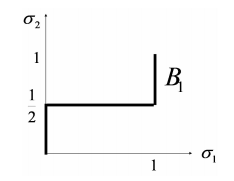
\includegraphics[width=100px]{./Kop_Zahl_BA.png}
\caption{Beste-Antworten beider Spieler 1}
\end{figure}
\subsection{Das Nash-Gleichgewicht}
\label{sec:org3534a51}
\subsubsection{NashGG in reinen Strategien}
\label{sec:org353abc6}
Mit dem Nash-GG kann man die Menge der Antworten noch weiter einschränken als durch das Aussortieren dominierter Strategien (denn die Strategie eines Nash-GG) wird nie (strikt) dominiert.\\
S ist ja die Menge der Strategiekombinationen, darin enthalten zB \{Hase, Hase\} oder \{RS, SS\}. Als \(s^* = (s^*_1, s^*_2, s^*_3, s^*_4) \epsilon S\) wird dann ein Nash-GG(in reinen Strategien) gekennzeichnet, wenn für alle i \(\le\) n gilt \\
\begin{equation*}
\begin{aligned}
s^*_i \epsilon B_i(s^*_1)
\end{aligned}
\end{equation*}
Diese Formel besagt das s\(^{\text{*}}_{\text{i}}\), also die Strategie von Spieler i, in den optimalen Beste-Antworten auf alle Strategien der Gegenspieler also s\(^{\text{*}}_{\text{-i}}\) beinhaltet sein muss. Wenn dies für alle i also für alle Spieler der Fall ist, handelt es sich um ein NashGG. Zum Beispiel Nash-GG, in dem beide Jäger auf Hirsch gehen, denn:

\(B_{\textcolor{magenta}{1}}(\textcolor{blue}{Hirsch}) = \textcolor{magenta}{Hirsch}\)
und
\(B_{\textcolor{blue}{2}}(\textcolor{magenta}{Hirsch}) = \textcolor{blue}{Hirsch}\)

Wenn beide Jäger auf Hase gehen, ist das auch ein Nash-GG, denn:
\(B_{\textcolor{magenta}{1}}(\textcolor{blue}{Hase}) = \textcolor{magenta}{Hase}\)
und
\(B_{\textcolor{blue}{2}}(\textcolor{magenta}{Hase}) = \textcolor{blue}{Hase}\)

Die Strategiekombinationen (Hirsch,Hase) und (Hase, Hirsch) sind jedoch keine NashGGs.

\subsubsection{NashGG in gemischten Strategien}
\label{sec:orgff72a1e}
Gibt es bei dem Spiel Kopf oder Zahl etwa kein Gleichgewicht?! Wie bereits gelernt können auch gemischte Strategien beste Antworten sein und werden somit auch als NashGG zugelassen.
Siehte weiter oben:
\begin{center}
\begin{tabular}{c|c|c}
\textcolor{magenta}{Spieler 1}/\textcolor{blue}{Spieler 2} & \textcolor{blue}{Kopf}(\(\sigma_{\text{2}}\)) & \textcolor{blue}{Zahl}(1-\(\sigma_{\text{2}}\))\\
\hline
\textcolor{magenta}{Kopf}(\(\sigma_{\text{1}}\)) & (\textcolor{magenta}{1},\textcolor{blue}{-1}) & (\textcolor{magenta}{-1},\textcolor{blue}{1})\\
\textcolor{magenta}{Zahl}(1-\(\sigma_{\text{1}}\)) & (\textcolor{magenta}{-1},\textcolor{blue}{1}) & (\textcolor{magenta}{1},\textcolor{blue}{-1})\\
\end{tabular}
\end{center}

\[ B_1(\sigma_2) =\begin{cases} 
      0 & \sigma_2 < \frac{1}{2} \\
      [0;1] & \sigma_2 = \frac{1}{2} \\
      1 & \sigma_2 > \frac{1}{2} 
   \end{cases}
\]

\[ B_2(\sigma_1) =\begin{cases} 
      1 & \sigma_1 < \frac{1}{2} \\
      [0;1] & \sigma_1 = \frac{1}{2} \\
      0 & \sigma_1 > \frac{1}{2} 
   \end{cases}
\]
Was bedeutet das obige? Die Spieler 1,..,i wählen ihre erste Strategie mit der Wahrscheinlichkeit \(\sigma_{\text{i}}\) und dementsprechend die zweite mit der Wahrscheinlichkeit \(1 - \sigma_i\) . Da beide Spieler in Abhängigkeit von der Strategiewahl des jeweils anderen Spielers eine unterschiedlichen Nutzen erlangen, hängt ihre Beste-Antwort von der Wahrscheinlichkeit mit der der Gegenspieler seine Strategien wählt ab. Was bei B\(_{\text{i}}\) als erstes hinter der geschweiften Klammer steht ist also der optimale Wert für "Wahrscheinlichkeit" \(\sigma_{\text{i}}\) mit der man selber agieren sollte um den maximalen Nutzen zu erzielen. Das hängt vom jeweiligen Wert der Wahrscheinlichkeit des Gegenspielers ab.\\
Im obigen Beispiel ist die beste Antwort des ersten Spielers \(BA_1(\sigma_2)\) auf ein \(\sigma_2 < \frac{1}{2}\) (Wahrscheinlichkeit das Spieler 2 Kopf spielt) der Wert \textcolor{magenta}{0} für \(\textcolor{magenta}{\sigma_1}\), was wie man in der Tabelle sehen kann, bedeuten würde, dass er am besten Zahl spielt, denn \(\textcolor{magenta}{Zahl(1-\sigma_1)}\), also \(1-\textcolor{magenta}{0}\) = 100\% Wahrscheinlichkeit.
\begin{figure}[htbp]
\centering
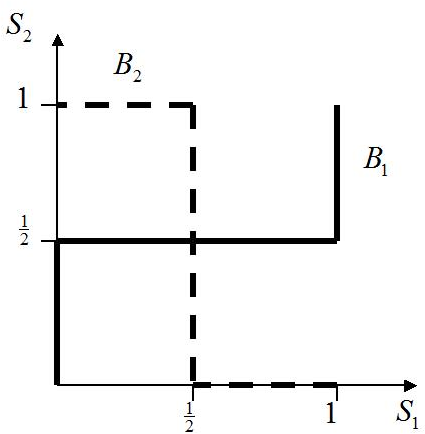
\includegraphics[width=100px]{./Kop_Zahl_BA2.png}
\caption{wechselseitig Beste-Antworten beider Spieler}
\end{figure}
\newline
NashGG's liegen dort, wo sich beide Funktionen schneiden in diesem Fall also bei \(\sigma_1=50\%\) , \(\sigma_2=50\%\) . Macht Sinn, denn bei anderer Wahrscheinlichkeit würde ein Spieler ja auch zu berechenbar werden. 

\paragraph{Polizeispiel}
\begin{center}
\begin{tabular}{c|c|c}
\textcolor{magenta}{Behörde}/\textcolor{blue}{Straftäter} & \textcolor{blue}{Betrug}(\(\sigma_{\text{2}}\)) & \textcolor{blue}{kein B.}(1-\(\sigma_{\text{2}}\))\\
\hline
\textcolor{magenta}{Kontrolle}(\(\sigma_{\text{1}}\)) & (\textcolor{magenta}{4-C},\textcolor{blue}{1-F}) & (\textcolor{magenta}{4-C},\textcolor{blue}{0})\\
\textcolor{magenta}{keine K.}(1-\(\sigma_{\text{1}}\)) & (\textcolor{magenta}{0},\textcolor{blue}{1}) & (\textcolor{magenta}{4},\textcolor{blue}{0})\\
\end{tabular}
\end{center}
In (Nash-)Gleichgewichten in gemischten Strategien sind alle Spieler indifferent zwischen den Handlungsalternativen.\\
Nutzen der Behörde bei Kontrolle: \(4-C\) \\
Nutzen der Behörde ohne Kontrolle: \(\sigma_2 * 0 + (1- \sigma_2)*4\) \\
Behörde also indifferent, wenn der Nutzen beider Strategien gleich ist:\\
\(4-C=\sigma_2 * 0 + (1- \sigma_2)*4\) \(\rightarrow\) Indifferent bei \(\sigma_2 = \frac{C}{4}\) .\\
\newline
Nutzen des Straftäters bei Betrug: \(\sigma_1 * (1-F) + (1-\sigma_1) * 1\) \\
Nutzen des Straftäters ohne Betrug: \(0\) \\
Straftäter also indifferent, wenn der Nutzen beider Strategien gleich ist:\\
\(\sigma_1 * (1-F) + (1-\sigma_1) * 1 = 0\) \(\rightarrow\) Indifferent bei \(\sigma_1 = \frac{1}{4}\)

\paragraph{Polizeispiel}
\textbf{Satz von Nash:} jedes endliche Spiel hat mind. ein GLeichgewicht, wenn man gemischte Strategien zulässt\\
\textbf{Satz von Wilson:} fast alle endlichen Spiele haben eine endliche, ungerade Anzahl von Gleichgewichten.
\subsection{Dynamische Spiele bei perfekter Information}
\label{sec:org5e91f6f}
Annahme, dass perfekte Informationen (alle bisherigen Spielzüge bekannt) bekannt sind und keine Züge der Natur vorliegen (aber auch leicht erweiterbar auf Spiele mit Zügen der Natur)
\paragraph{Ultimatum-Spiel:}
\begin{itemize}
\item Aufteilung von drei Münzen zwischen zwei Spielern
\item Spieler 1 macht einen Vorschlag, Spieler 2 nimmt an oder lehnt ab
\item Bei Ablehnung bekommt keiner der Spieler etwas
\item Keine Nachverhandlungen
\end{itemize}
\begin{center}
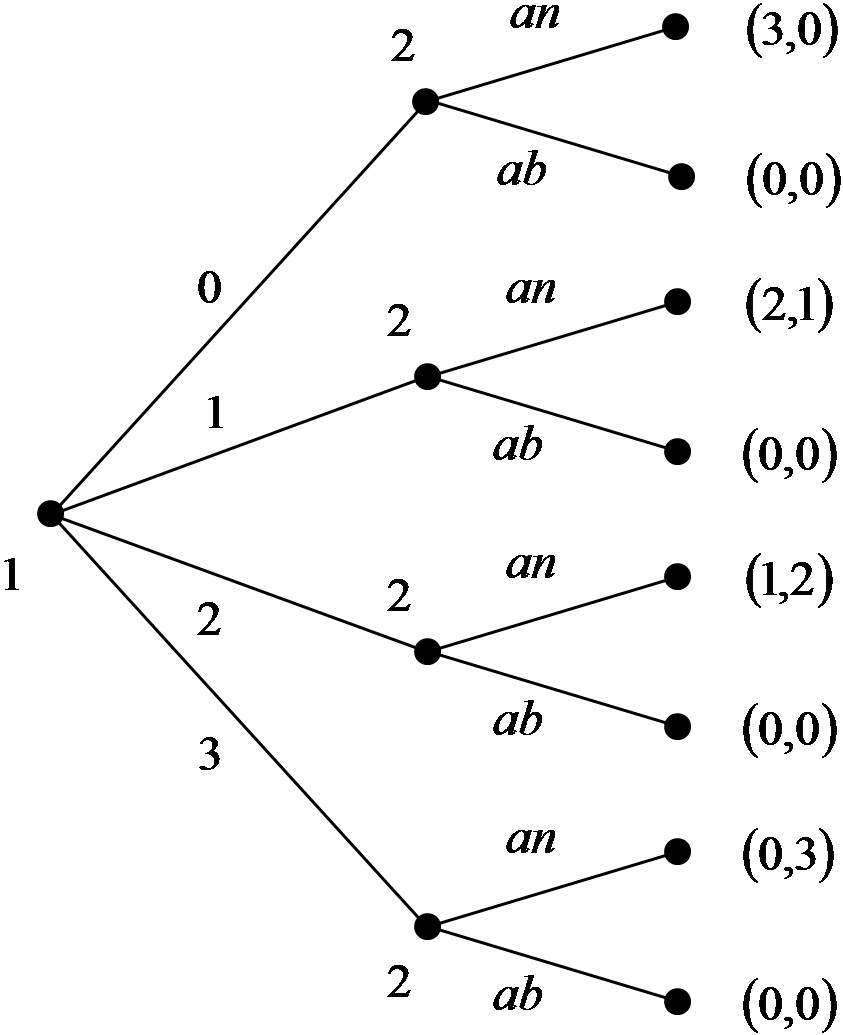
\includegraphics[width=100px]{./urbaum.png}
\end{center}

\textbf{eine} Strategie = eine Vorschrift, die an \textbf{jedem Knoten} eine Entscheidung festlegt;*vollständiger* Plan eines Spielers, was zu tun ist\\
Strategien Spieler 1: [0],[1],[2],[3]\\
Strategien Spieler 2: alle Reaktionen auf alle möglichen Angebote, \textbf{eine} beispielhafte Strategie = [0] annehmen, [1] annehmen, [2] ablehnen, [3] ablehnen

Menge der Strategien von S2 = 2\(^{\text{4}}\) (=16) also die eigenen Reaktionsmöglichkeiten (annehmen, ablehnen) hoch die Strategienanzahl von Spieler 1 (4), zB:
\begin{center}
\begin{tabular}{l}
(an, an, an, an)\\
(an, an, an, ab)\\
(an, an, ab, an)\\
(an, ab, an, an)\\
\ldots{}\\
\end{tabular}
\end{center}
Die strategische Form bildet all diese Strategien mit ihren Auszahlungen in einer Matrix ab
\begin{center}
\begin{tabular}{rllllll}
S1 $\backslash$ S2 & an,an,an,an & an,an,an,ab & an,an,ab,an & an,ab,an,an & \ldots{} & ab,ab,ab,ab\\
\hline
0 & (3,0) & (3,0) & (3,0) & (3,0) & \ldots{} & (0,0)\\
1 & (2,1) & (2,1) & (2,1) & (2,0) & \ldots{} & (0,0)\\
2 & (1,2) & (1,2) & (1,0) & (1,2) & \ldots{} & (0,0)\\
3 & (0,3) & (0,0) & (0,3) & (0,3) & \ldots{} & (0,0)\\
\end{tabular}
\end{center}
Hier ist ebenfalls die Rückwärtsinduktion beim Baum hilfreich um das Spiel zu lösen. Wenn man alle letzten Teilbäume betrachtet fällt schonmal auf das [ab,ab,ab,ab] also "ab" auf jedes Angebot nicht optimal ist \(\rightarrow\) kann somit gestrichen werden. Wiederholt man diesen Prozess des Vergleichens in der oberen Tabelle, verbleiben letztendlich nur noch [an,an,an,an] und [ab,an,an,an] als gleichwertig optimale Strategien fuer Spieler 2.\\
Spieler 1 braucht also nur noch diese beiden Strategien von Spieler 2 in Betracht ziehen und genau diese beiden Gleichgewichte sind auch teilspielperfekt. Ein teilspielperfektes Gleichgewicht ist ein NashGG das auch auf jedem Teilspiel ein NashGG ist.
\begin{center}
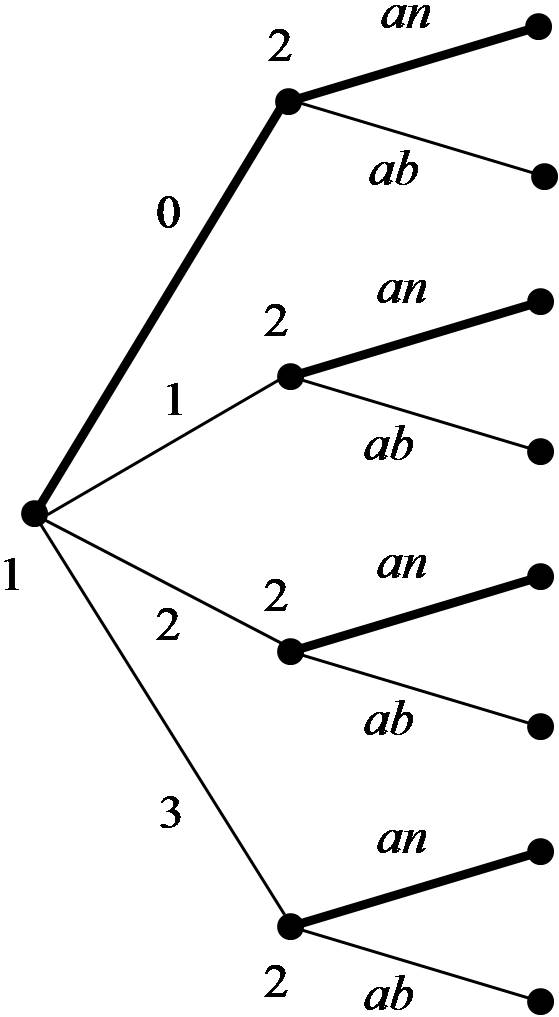
\includegraphics[height=0.4\textwidth]{./4an.png}
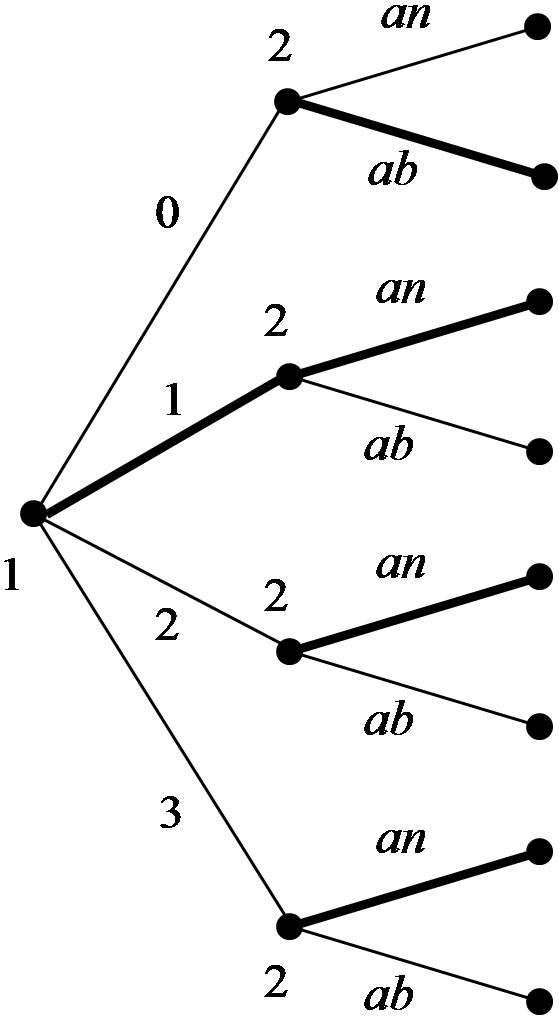
\includegraphics[height=0.4\textwidth]{./3an.png}
\end{center}

\subsection{Dynamische Spiele bei imperfekter Information}
\label{sec:org5108eee}
Züge der Natur sind ein möglicher Grund für imperfekte Information(möglicherweise asymmetrisch verteilte Information)
\(\rightarrow\) siehe F.120 / S.129
\paragraph{Bayes'sches Gleichgewicht}
Anfangs entsprechen die Informationsstände der Spieler den von der Natur vergegeben Wahrscheinlichkeiten.\\
Beispiel: Die Wahrsch. eines 1-Euro-“Typen” ist 50\%.
Aber bei längeren/dynamischen Spielen können Spieler durch ihre Entscheidungen ihren Typen (teilweise) offenbaren (zB Bieter bei einer offenen Auktion der seine eigene Zahlungsbereitschaft=Typ über die Gebote hinweg tlw. offenbart).\\
In einem \textbf{perfekten Bayes'schen Gleichgewicht}:
\begin{enumerate}
\item sind die Strategien der Spieler jederzeit optimal, gegeben die aktuellen Informationsstände
\item werden die Informationsstände jederzeit rational aktualisiert
\end{enumerate}

\section{Notes}
\label{sec:orgd177f5e}
\begin{enumerate}
\item z \(\epsilon\) Z bedeutet alle anderen Variablen zum Beispiel s\(_{\text{1}}\) konstant zu halten und die Auszahlungen fuer alle z zu betrachten
\item ableitungsregeln, partielle ableitung, ableitung von spezialfaellen, bruch in wurzel schreiben
\end{enumerate}
\end{document}
